
\section{Overview of Human Action Recognition}
\begin{frame}{Overview of Human Action Recognition}
    Human action recognition can be divided into two phases: action classification and action detection.
    \begin{itemize}
        \item Action classification is the analysis of a segmented video containing only a single action that must be classified into a defined action category (early).
        \item Action detection detects the start and end times of each action in the video, locates their position in space, and identifies the action category (more challenging).
    \end{itemize}
\end{frame}

\begin{frame}{Overview of Human Action Recognition}
    Techniques can be categorized into the following four classes of action semantics from low to high:
    \begin{itemize}
        \item Primitive action recognition (waving, lifting a foot, bending).
        \item Single-person action recognition (walking, punching, jumping).
        \item Interaction recognition (playing an instrument, carrying a knife). It has received \textbf{more attention in recent years}.
        \item Group action recognition (parade, group meeting). It is \textbf{still in its infancy}.
    \end{itemize}
\end{frame}

\section{Applications}
\begin{frame}{Applications}
    Human action recognition has a wide range of a applications:

    \begin{itemize}
        \item Intelligent video surveillance.
        \item Environmental home monitoring.
        \item Video storage and retrieval.
        \item Intelligent human–machine interfaces.
        \item Identity recognition.
    \end{itemize}
\end{frame}

\section{Type of Dataset}
\begin{frame}{Type of Dataset}
    Most reviews of human action recognition are limited to approaches based on specific data:

    \begin{itemize}
        \item RGB data.
        \item Depth data.
        \item Skeleton data.
    \end{itemize}
\end{frame}

\begin{frame}{Type of Dataset}
    Skeleton and RGB and Depth sample frames from the NTU RGB+D Human Activity Dataset \cite{shahroudy2016ntu}.
    \begin{multicols}{2}
        \begin{figure}[htp]
            \centering
            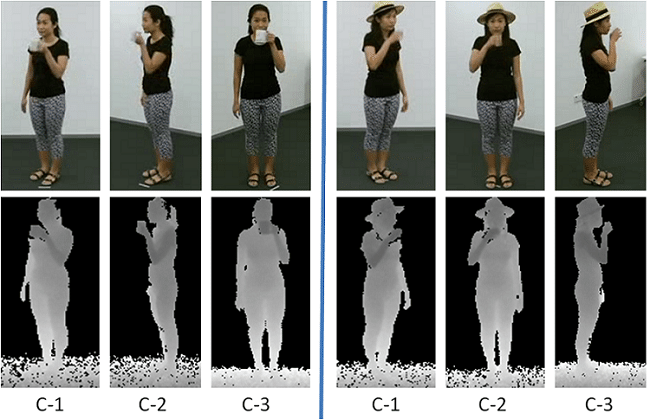
\includegraphics[height=3cm]{images/v1survey/depth_data_ex.png}
            \caption{Depth data}
            \label{fig:depth_data_ex}
        \end{figure}
        \begin{figure}[htp]
            \centering
            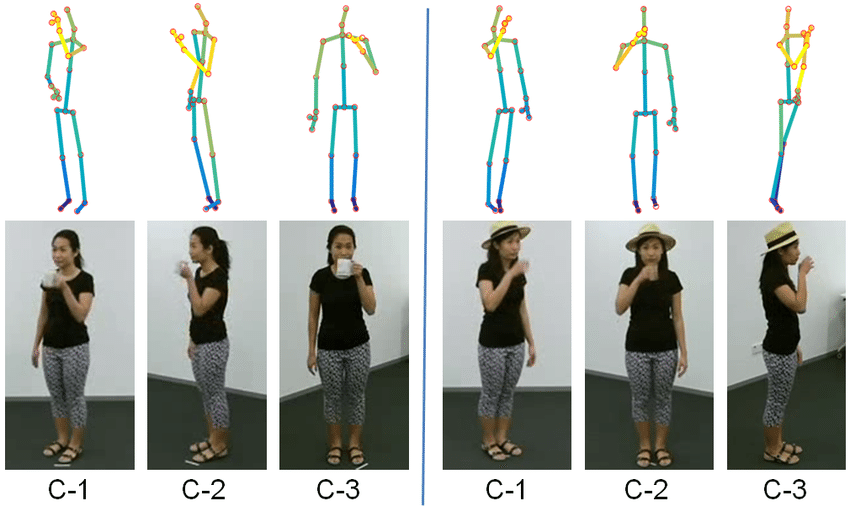
\includegraphics[height=3cm]{images/v1survey/skeleton_data_ex.png}
            \caption{Skeleton data}
            \label{fig:skeleton_data_ex}
        \end{figure}
    \end{multicols}
\end{frame}

\section{Feature representation}
\subsection{Handcrafted Action Features}
\begin{frame}{Feature representation}
    \begin{itemize}
        \item The problem of feature representation in HAR is extended from two-dimensional space to three-dimensional space-time.
        \item In recent years, many kinds of action representation methods have been proposed:
              \begin{enumerate}
                  \item Action Features for RGB Data.
                  \item Action Features for Depth and Skeleton Data.
                  \item Feature Fusion methods.
              \end{enumerate}
    \end{itemize}
\end{frame}

\begin{frame}{Handcrafted Action Features (RGB)}
    \begin{itemize}
        \item<1-> Spatiotemporal volume-based action representation methods (\href{https://web.cse.ohio-state.edu/~davis.1719/CVL/Research/MHI/mhi.html}{motion history image, motion energy image}) \cite{li2011human}.
              \only<1>{
                  \begin{figure}[htp]
                      \centering
                      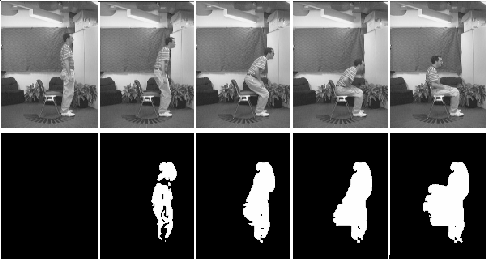
\includegraphics[height=2cm, width=7cm]{images/v1survey/mei.png}
                      \caption{Motion history image}
                  \end{figure}
                  \begin{figure}[htp]
                      \centering
                      \includegraphics<1>[height=2cm, width=7cm]{images/v1survey/mhi.png}
                      \caption{Motion energy image}
                  \end{figure}
              }
              % [Global features] The camera is fixed  -> background subtraction techniques
              % -> shape information (silhouettes and contours) -> key template matrix -> matching
        \item<2-> STIP-based methods (Feature descriptors: SIFT, HOG) \cite{nguyen2014stap}.
              \only<2>{
                  \begin{figure}[htp]
                      \centering
                      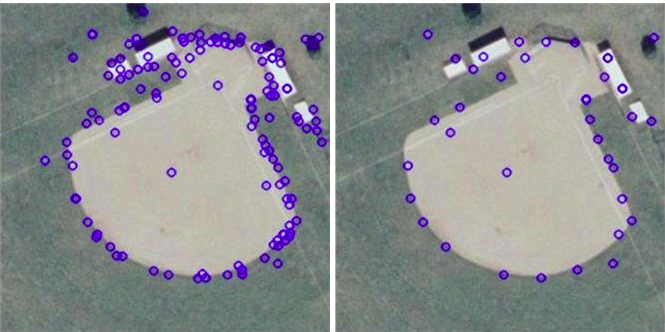
\includegraphics[width=0.45\textwidth]{images/v1survey/sift.png}
                      \caption{Scale-invariance feature transform}
                  \end{figure}
              }
              % [Local features] key region of movement change.
        \item<3-> Action representation methods based on the trajectory of skeleton joints (Gunner Farneback’s algorithm, Lucas-Kanade and corners detected using Shi-Tomasi algorithm).
              % tracking path of key points or the joints in the human skeleton
    \end{itemize}
\end{frame}

\begin{frame}{Handcrafted Action Features \\ (Depth, Skeleton)}
    \begin{itemize}
        \item Good human detection and pose estimation performance has been achieved using depth data (DMM, EHOG).
        \item From depth data, the human skeleton can be estimated quickly and accurately (3DHOG, AME).
        \item Research results show that the methods based on depth information achieve real-time action recognition and better recognition performance than RGB-based methods.
    \end{itemize}
\end{frame}

\subsection{Methods Based on Deep Learning}
\begin{frame}{Methods Based on Deep Learning}
    \begin{itemize}
        \item In recent years, the application of deep learning to computer vision has received considerable attention.
        \item Many deep learning-based action representation methods have been proposed in the field of human action recognition
              \begin{itemize}
                  \item Two-stream convolutional networks.
                  \item 3D convolutional networks.
                  \item Long short-term memory (LSTM).
              \end{itemize}
    \end{itemize}
\end{frame}

\begin{frame}{Two-stream convolutional networks}
    What is the approach used by the authors?
    \begin{itemize}
        \item Spatial network
        \item Temporal stream network
    \end{itemize}
    \begin{figure}[htp]
        \centering
        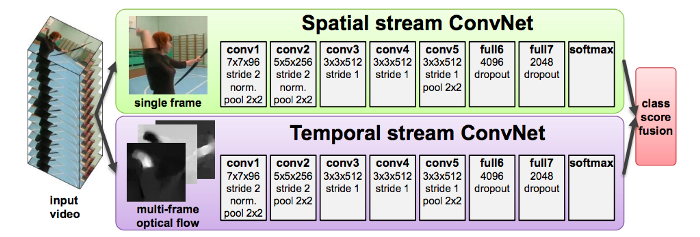
\includegraphics[width=0.8\textwidth]{images/v1survey/2-stream-cnn.png}
        \caption{Two-stream convolutional networks}
    \end{figure}
\end{frame}

\begin{frame}{3D convolutional networks}
    \begin{figure}[htp]
        \centering
        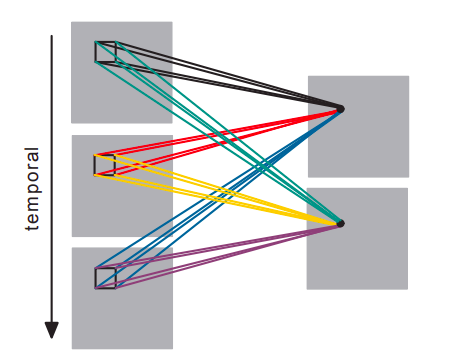
\includegraphics[width=0.8\textwidth]{images/v1survey/3d-cnn.png}
        \caption{3D convolutional networks}
    \end{figure}
\end{frame}

\begin{frame}[allowframebreaks]
    \frametitle{Long short-term memory (LSTM)}
    \begin{figure}[htp]
        \centering
        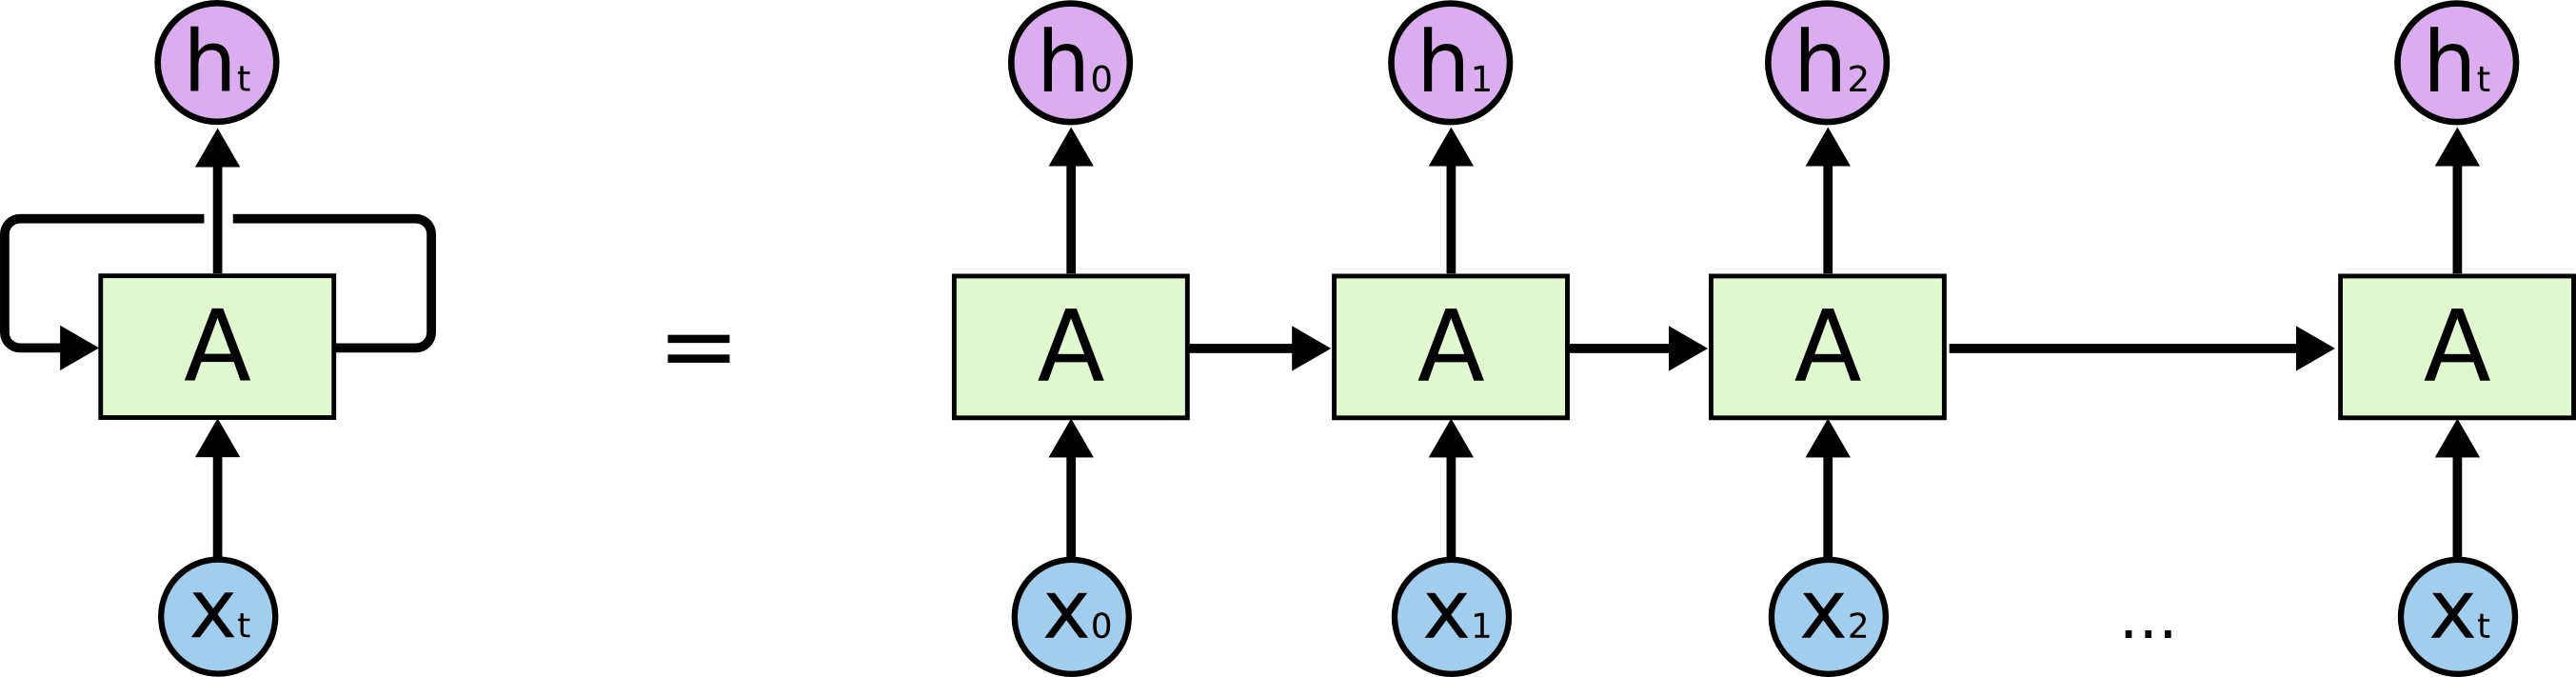
\includegraphics[width=\textwidth]{images/v1survey/RNN-unrolled.png}
        \caption{RNN}
    \end{figure}
    \begin{figure}[htp]
        \centering
        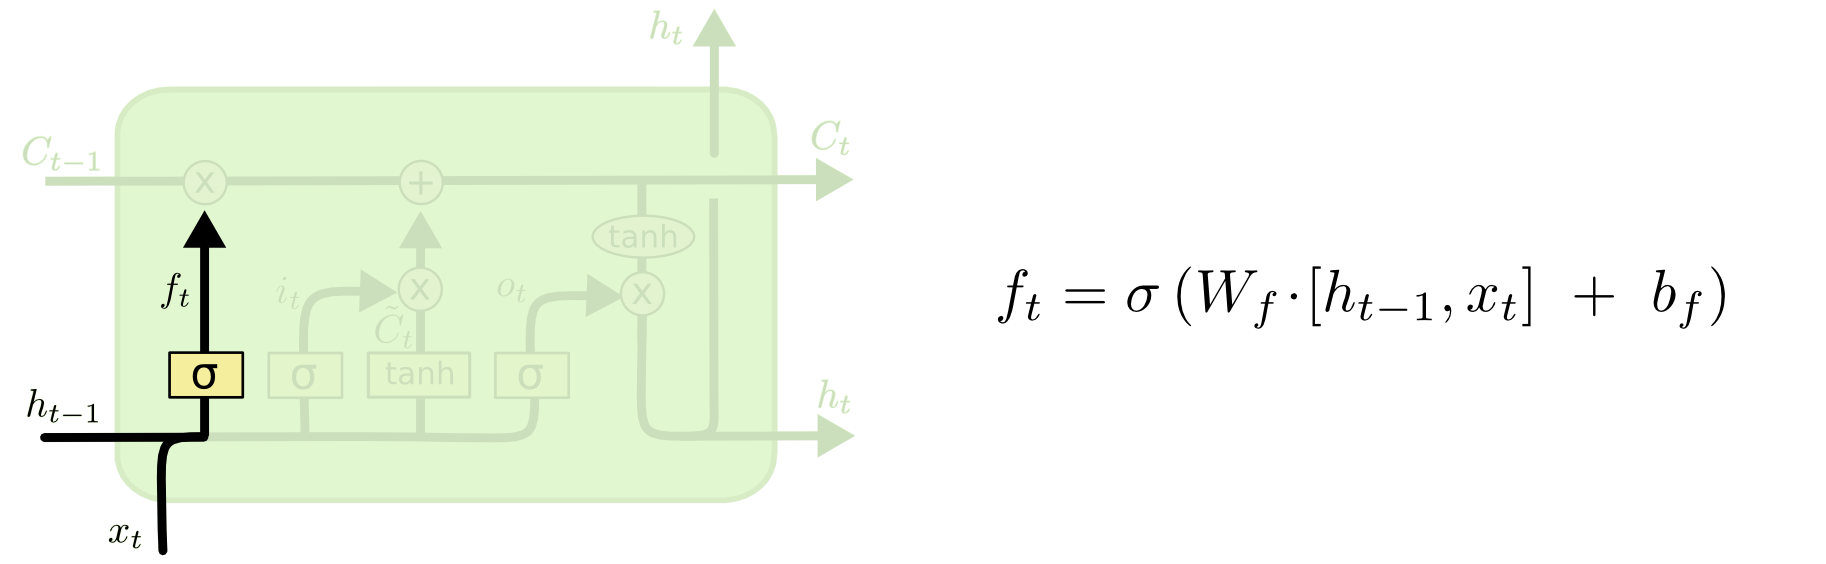
\includegraphics[width=\textwidth]{images/v1survey/LSTM-1.png}
        \caption{Forget gate layer (Sigmoid)}
    \end{figure}
    \begin{figure}[htp]
        \centering
        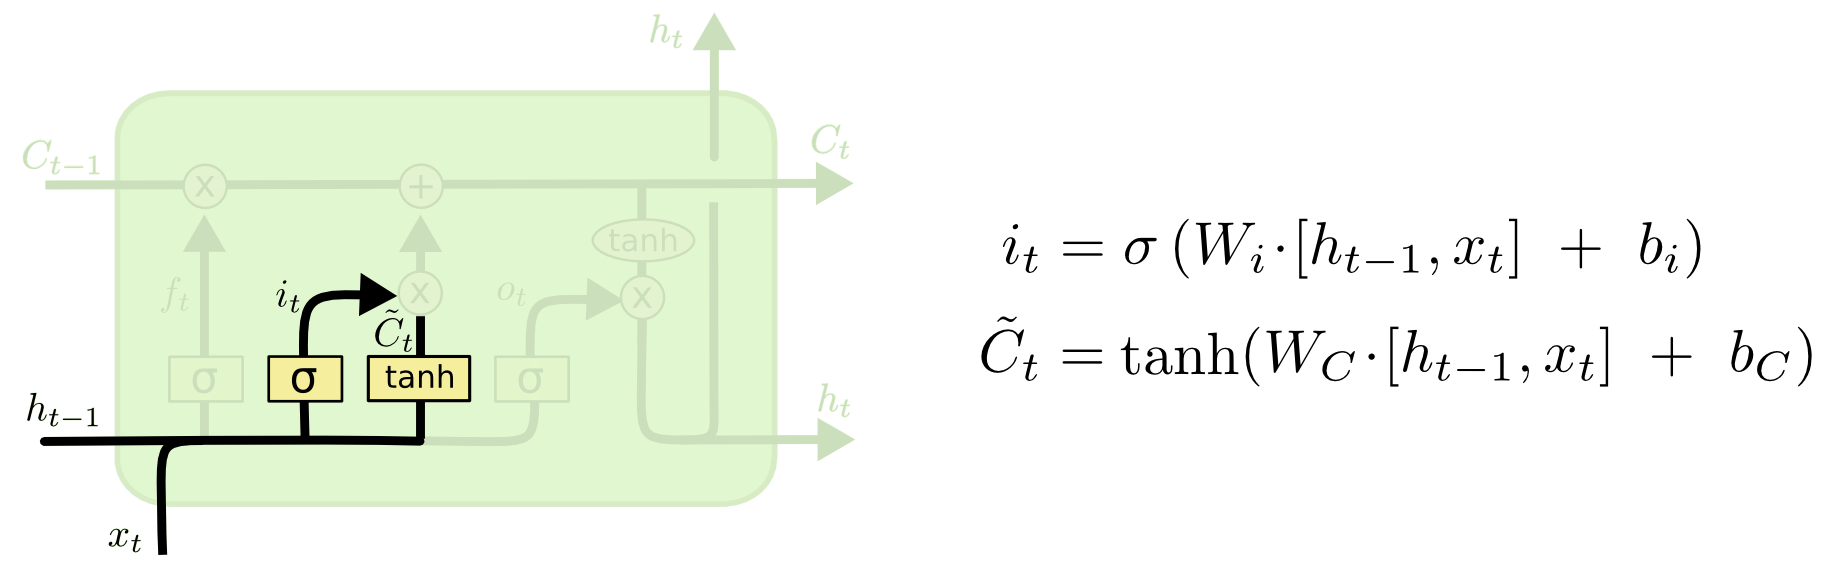
\includegraphics[width=\textwidth]{images/v1survey/LSTM-2.png}
        \caption{Input gate layer (Tanh, Sigmoid)}
    \end{figure}
    \begin{figure}[htp]
        \centering
        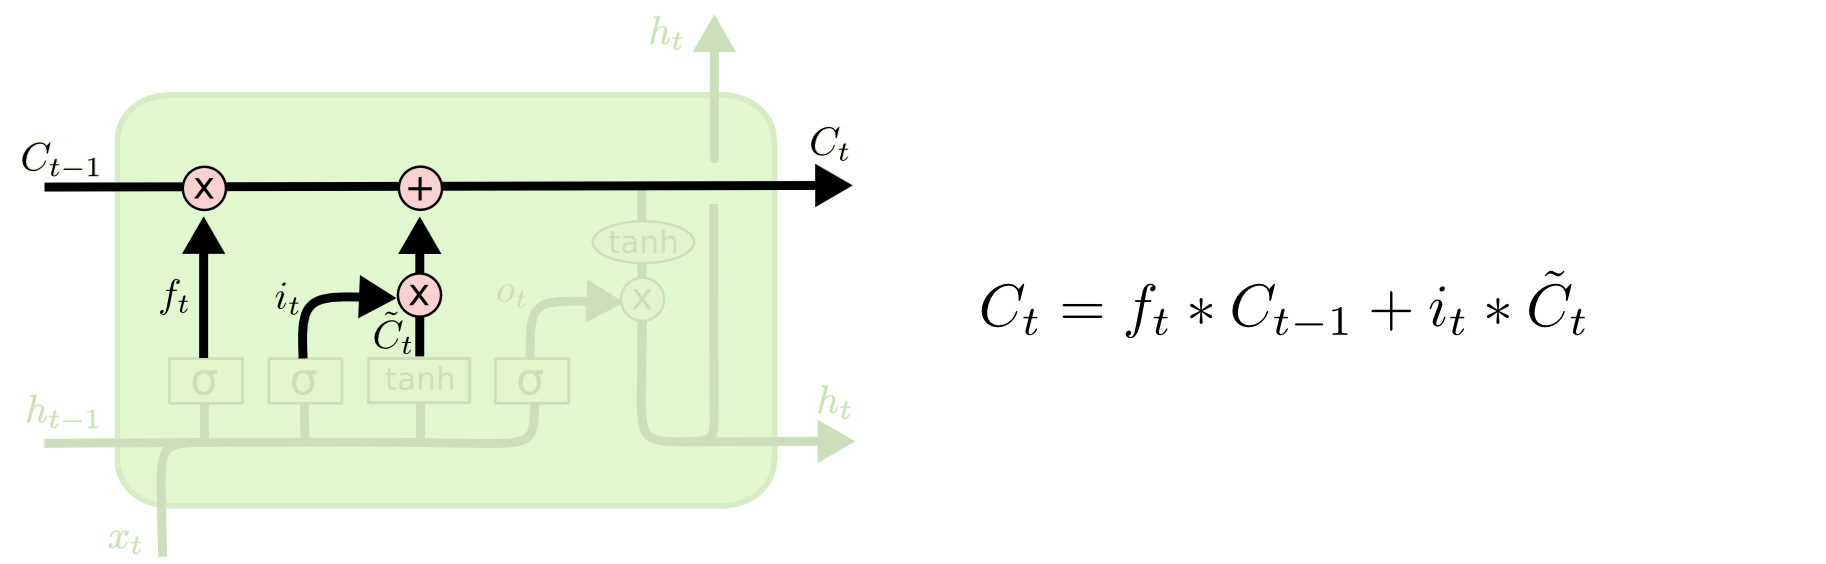
\includegraphics[width=\textwidth]{images/v1survey/LSTM-3.png}
        \caption{Update gate layer}
    \end{figure}
    \begin{figure}[htp]
        \centering
        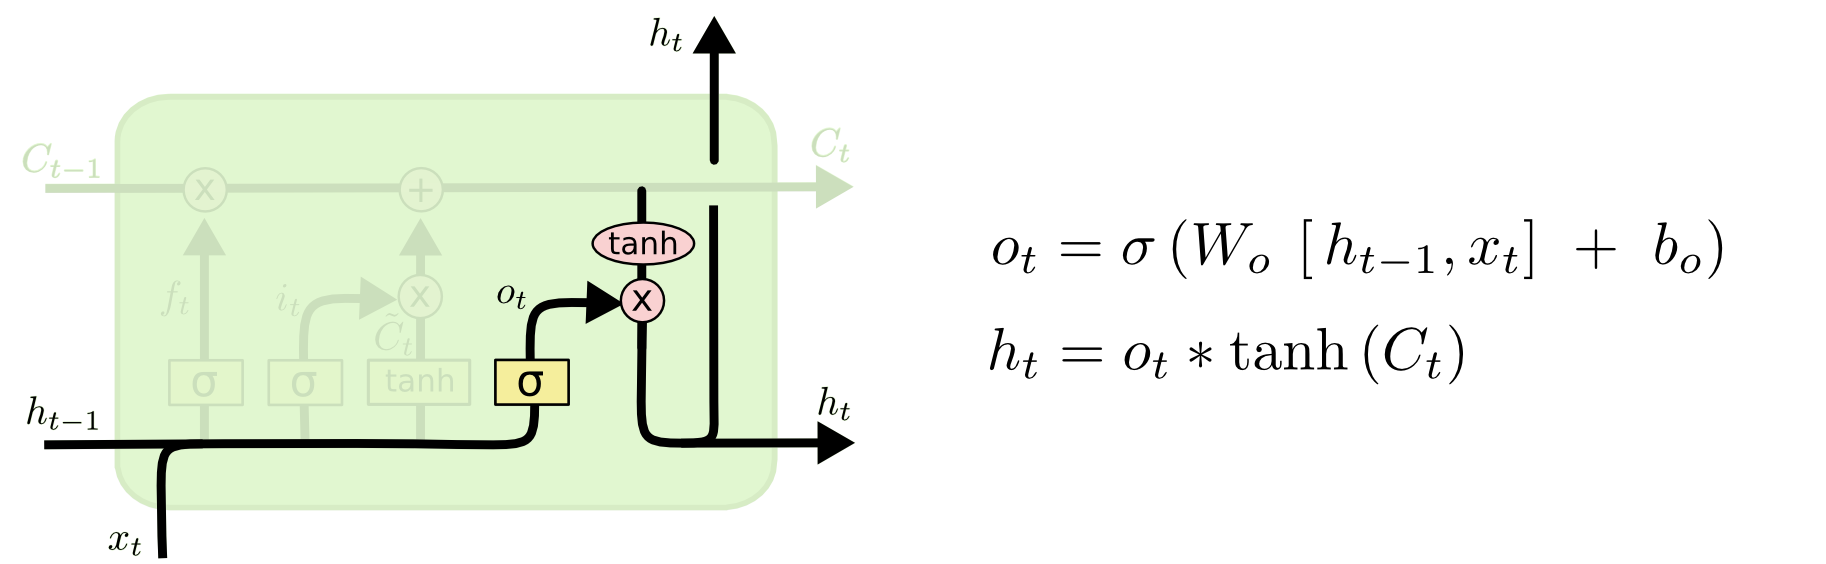
\includegraphics[width=\textwidth]{images/v1survey/LSTM-4.png}
        \caption{Output gate layer}
    \end{figure}
\end{frame}